\documentclass[10pt]{beamer}

\usetheme[progressbar=frametitle]{metropolis}
\usepackage{appendixnumberbeamer}

\usepackage{booktabs}
\usepackage[scale=2]{ccicons}

\usepackage{pgfplots}
\usepgfplotslibrary{dateplot}

\usepackage{xspace}
\newcommand{\themename}{\textbf{\textsc{metropolis}}\xspace}

\title{Dynamic Control Systems}
\subtitle{Lecture 1 - Introduction to Linear Systems}
% \date{\today}
\date{}
\author{Prof. Engr. Nikolay Prieto Ph.D.(c)}
\institute{Escuela Colombiana de Carreras Industriales - ECCI}
\titlegraphic{\hfill
\includegraphics[height=1.5cm]{pr-aaaaecci.jpg}}

\begin{document}

\maketitle

\begin{frame}{Why System Control Dynamics?}
\begin{figure}
    \centering
    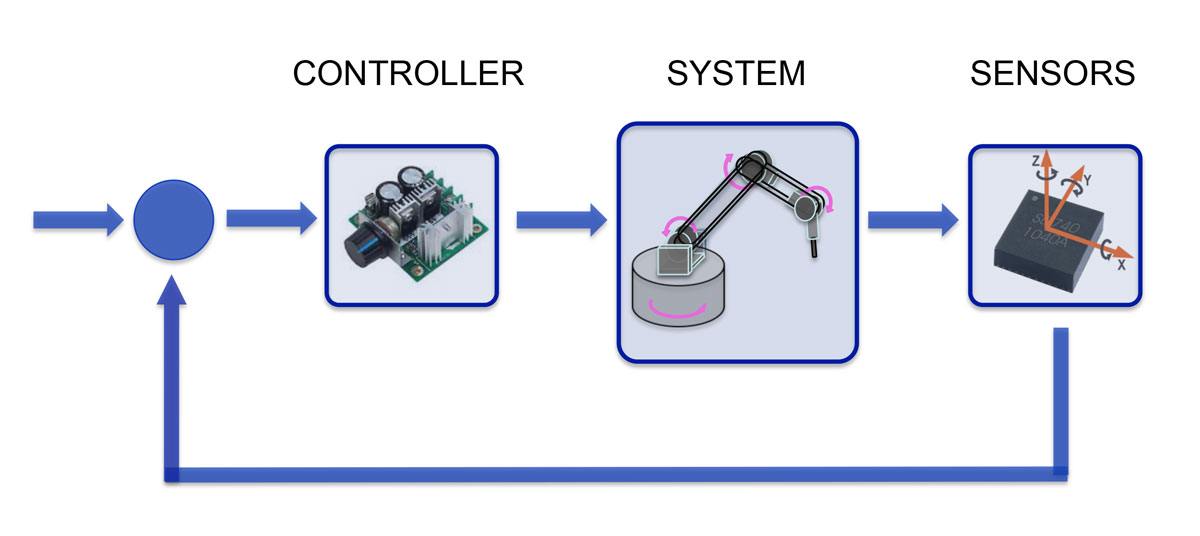
\includegraphics[scale=0.2]{loop.jpg}
    \caption{Closed loop robotic system }
    \label{fig:my_label1}
\end{figure}
    
\end{frame}

\begin{frame}[fragile]{Pre-requisites and Requirements}
  \begin{columns}[T,onlytextwidth]
    \column{0.5\textwidth}
      Fields
  	\begin{itemize}[<+- | alert@+>]
    % \item \alert<4>{This is\only<4>{ really} important}
    \item Aeronautics.
    \item Automatic control Systems.
    \item Economics, finance.
    \item Circuit analysis, simulations.
    \item Mechanical and civil engineering.
  	\end{itemize}

    \column{0.5\textwidth}
	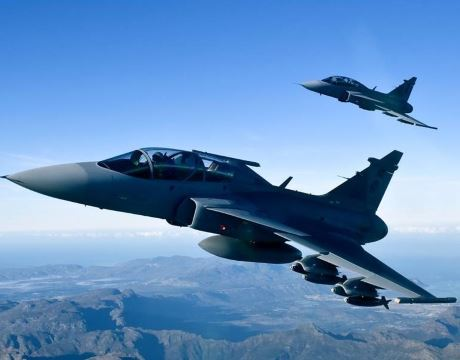
\includegraphics[scale=0.4]{aeronautics.jpg}}
  \end{columns}
\end{frame}

\begin{frame}{Linear Systems}

    \begin{alertblock}{Statement}
        If you do not understand linear dynamical systems, you certainly cannot understand Non linear systems.
    \end{alertblock}
    \begin{block}{Advantages}
    \begin{itemize}
        \item Methods for linear systems often work --- unreasonably well --- in practice
        \item Most techniques for non linear systems are based linear methods.
    \end{itemize}
    \end{block}
    
\end{frame}

\begin{frame}{Example}
\begin{columns}[T,onlytextwidth]
\column{0.5\textwidth}
\begin{figure}
    \centering
    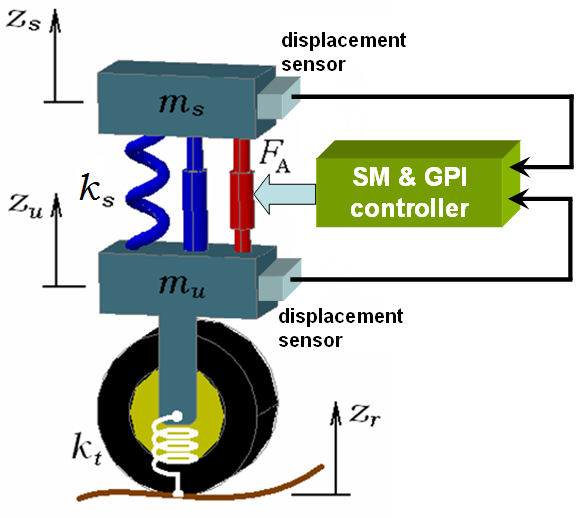
\includegraphics[scale=0.2]{controlSuspension.png}
    \caption{Car Suspension System Control}
    \label{fig:my_label2}
\end{figure}
\column{0.5\textwidth}
\begin{figure}
    \centering
    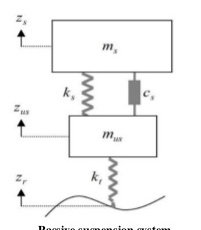
\includegraphics[scale=2.0]{suspension.jpg}
    \caption{Model Simplified}
    \label{fig:my_label3}
\end{figure}
\end{columns}
\end{frame}

\begin{frame}[fragile]{Pre-requisites and Requirements}
    \begin{itemize}
        \item Exposure to Linear Algebra
        \item Exposure to Laplace Transform, Differential Equations
        \item Circuits \& systems
        \item Dynamics 
    \end{itemize}

    % Imported from lyx
    
    \begin{table}
    \begin{centering}
    \begin{tabular}{|c|c|c|c|}
    \hline 
     & Init Term (30\%) & Mid Term(30\%) & Final Term(30\%)\tabularnewline
    \hline 
    \hline 
    Quizzes and others & 33\% & 33\% & 25\%\tabularnewline
    \hline 
    Project & 17\% & 17\% & 25\%\tabularnewline
    \hline 
    Exam & 50\% & 50\% & 50\%\tabularnewline
    \hline 
    \end{tabular}
    \par\end{centering}
    \caption{Course requirements.}
    \end{table}

\end{frame}

\end{document}
